%%%%%%%%%%%%%%%%%%%%%%%%%%%%%%%%%%%%%%%%%%%%%%%%%%%%%%%%%%%%%%%%%%%%%%%%%%%%%%%
\section{CONCEPTUAL DESIGN}
%%%%%%%%%%%%%%%%%%%%%%%%%%%%%%%%%%%%%%%%%%%%%%%%%%%%%%%%%%%%%%%%%%%%%%%%%%%%%%%

%TODO SOME TEXT HERE!!

%%%%%%%%%%%%%%%%%%%%%%%%%%%%%%%%%%%%%%%%%%%%%%%%%%%%%%%%%%%%%%%%%%%%%%%%%%%%%%%
\subsection{Methodology} \label{sec:ConceptualDesignMethodology}
%%%%%%%%%%%%%%%%%%%%%%%%%%%%%%%%%%%%%%%%%%%%%%%%%%%%%%%%%%%%%%%%%%%%%%%%%%%%%%%

The conceptual design methodology for solar-powered UAVs used in this paper was developed at ETH Zurich in~\cite{Noth_PhD,Leutenegger_JIRS} and is briefly summarized below. To analyze flight performance and a potential perpetual flight capability, the energy input/output-balance needs to be modeled. The total required nominal electrical output power
\begin{equation} \label{eqn:P_out}
P_{out}^{\,nom}=\frac{P_{level}}{\eta_{prop}}+P_{av}+P_{pld}
\end{equation}
consists of the required electrical propulsion power for level-flight $\frac{P_{level}}{\eta_{prop}}$ , where $\eta_{prop}$ includes propeller, gearbox, motor, and motor-controller efficiency, and the necessary avionics and payload power $P_{av}$ and $P_{pld}$. The UAV is assumed to fly at the airspeed of minimum aerodynamic level-flight power
\begin{equation} \label{eqn:P_level}
P_{level}=\left(\frac{C_D}{C_L^\frac{3}{2}}\right)_{min}\sqrt{\frac{2(m_{tot}g)^3}{\rho(h)A_{wing}}} .
\end{equation}
Here, $m_{tot}=m_{bat}+m_{struct}+m_{prop}+m_{sm}+m_{av}+m_{pld}$ is the total airplane mass, where structure, propulsion and solar module masses $m_{struct}$, $m_{prop}$, $m_{sm}$ are automatically sized according to \cite{Noth_PhD,Leutenegger_JIRS} and $m_{av}$, $m_{pld}$ are given in Table~\ref{tab:ConceptDesignParameters}. The local earth gravity is designated by $g$, $A_{wing}$ is the wing area, and $\rho(h)$ is the altitude dependent air density. The airplane lift and drag coefficients $C_L$ and $C_D$ are retrieved from 2-D airfoil simulations using XFoil \cite{Drela_XFoil}, with $C_D$ being combined with parasitic drag from the airplane fuselage and stabilizers and the induced drag  
\begin{equation} \label{eqn:C_D}
C_{D,ind}=\frac{c_L^2}{\pi\cdot e_0\cdot\lambda} .
\end{equation}
Here, $e_0\approx0.92$ is the Oswald efficiency and $\lambda$ the wing aspect ratio. On the input side, the nominal solar input power
\begin{equation} \label{eqn:P_solar}
P_{solar}^{\,nom}=I\cdot A_{sm}\cdot\eta_{sm}\cdot\eta_{mppt}
\end{equation}
considers the solar module area $A_{sm}=f_{sm}\cdot A_{wing}$ with relative fill-factor $f_{sm}$, module efficiency $\eta_{sm}$, and Maximum Power Point Tracker (MPPT) efficiency $\eta_{mppt}$. The solar radiation $I=I(\varphi,h,t)$ is assumed to be a function of the geographical latitude $\varphi$, the altitude $h$, and the current date and local time $t$, and is modeled as in \cite{Duffie_SolarEngineering}.
The state equation is now
\begin{equation}\label{eqn:StateEquations}
\begin{array}{r@{}l}
\frac{dE_{bat}}{dt}&=P_{solar}(\varphi,h,t)-u-P_{av}-P_{pld},\\
\frac{dh}{dt}&=\frac{\eta_{prop}\cdot u-P_{level}(h)}{m_{tot}g} .
\end{array}
\end{equation}
Here, $u$ is the current electrical power sent to the propulsion system and $P_{solar}$ denotes the incoming solar power. By solving the system of differential equations in (\ref{eqn:StateEquations}), the energy stored in the batteries may be obtained and thus the perpetual flight capability of the UAV determined.

For the design optimization, we assume that a solar-powered UAV configuration is designed for missions at and around a specific Date of the Year (DoY) and geographical latitude $\varphi$, thus $\varphi$ and $DoY$ are fixed. The three design parameters are a) wingspan $b$ and b) wing aspect ratio $\lambda$, which both specify wing geometry and thus influence level-power (\ref{eqn:P_level}) and solar input power (\ref{eqn:P_solar}), and c) the battery mass $m_{bat}$ contained in $m_{tot}$ in (\ref{eqn:P_level}) .

%%%%%%%%%%%%%%%%%%%%%%%%%%%%%%%%%%%%%%%%%%%%%%%%%%%%%%%%%%%%%%%%%%%%%%%%%%%%%%%
\subsection{Extension of Conceptual Design Optimization Criteria}
%%%%%%%%%%%%%%%%%%%%%%%%%%%%%%%%%%%%%%%%%%%%%%%%%%%%%%%%%%%%%%%%%%%%%%%%%%%%%%%

\label{sec:ExtensionOptCriteria}
The conceptual design tool developed in \cite{Noth_PhD,Leutenegger_JIRS} has been extended in two ways: First, it now provides the capability to perform energetic simulations of multi-day solar-powered flight, whereas before only one day-night cycle was considered. Figure \ref{fig:EnergySimulation} shows the results for incoming solar power $P_{solar}$, required power $P_{out}$, and remaining battery charge $E_{bat}$ obtained for a flight of two subsequent day-night cycles. Clearly, the initial charge condition $E_{bat}$ at time of sunrise $t_{sr}=\min(t(P_{solar}>0))$ for the second day is different than on the first day, which significantly influences the re-charging process. 
\begin{figure}[tb]
    \centering
    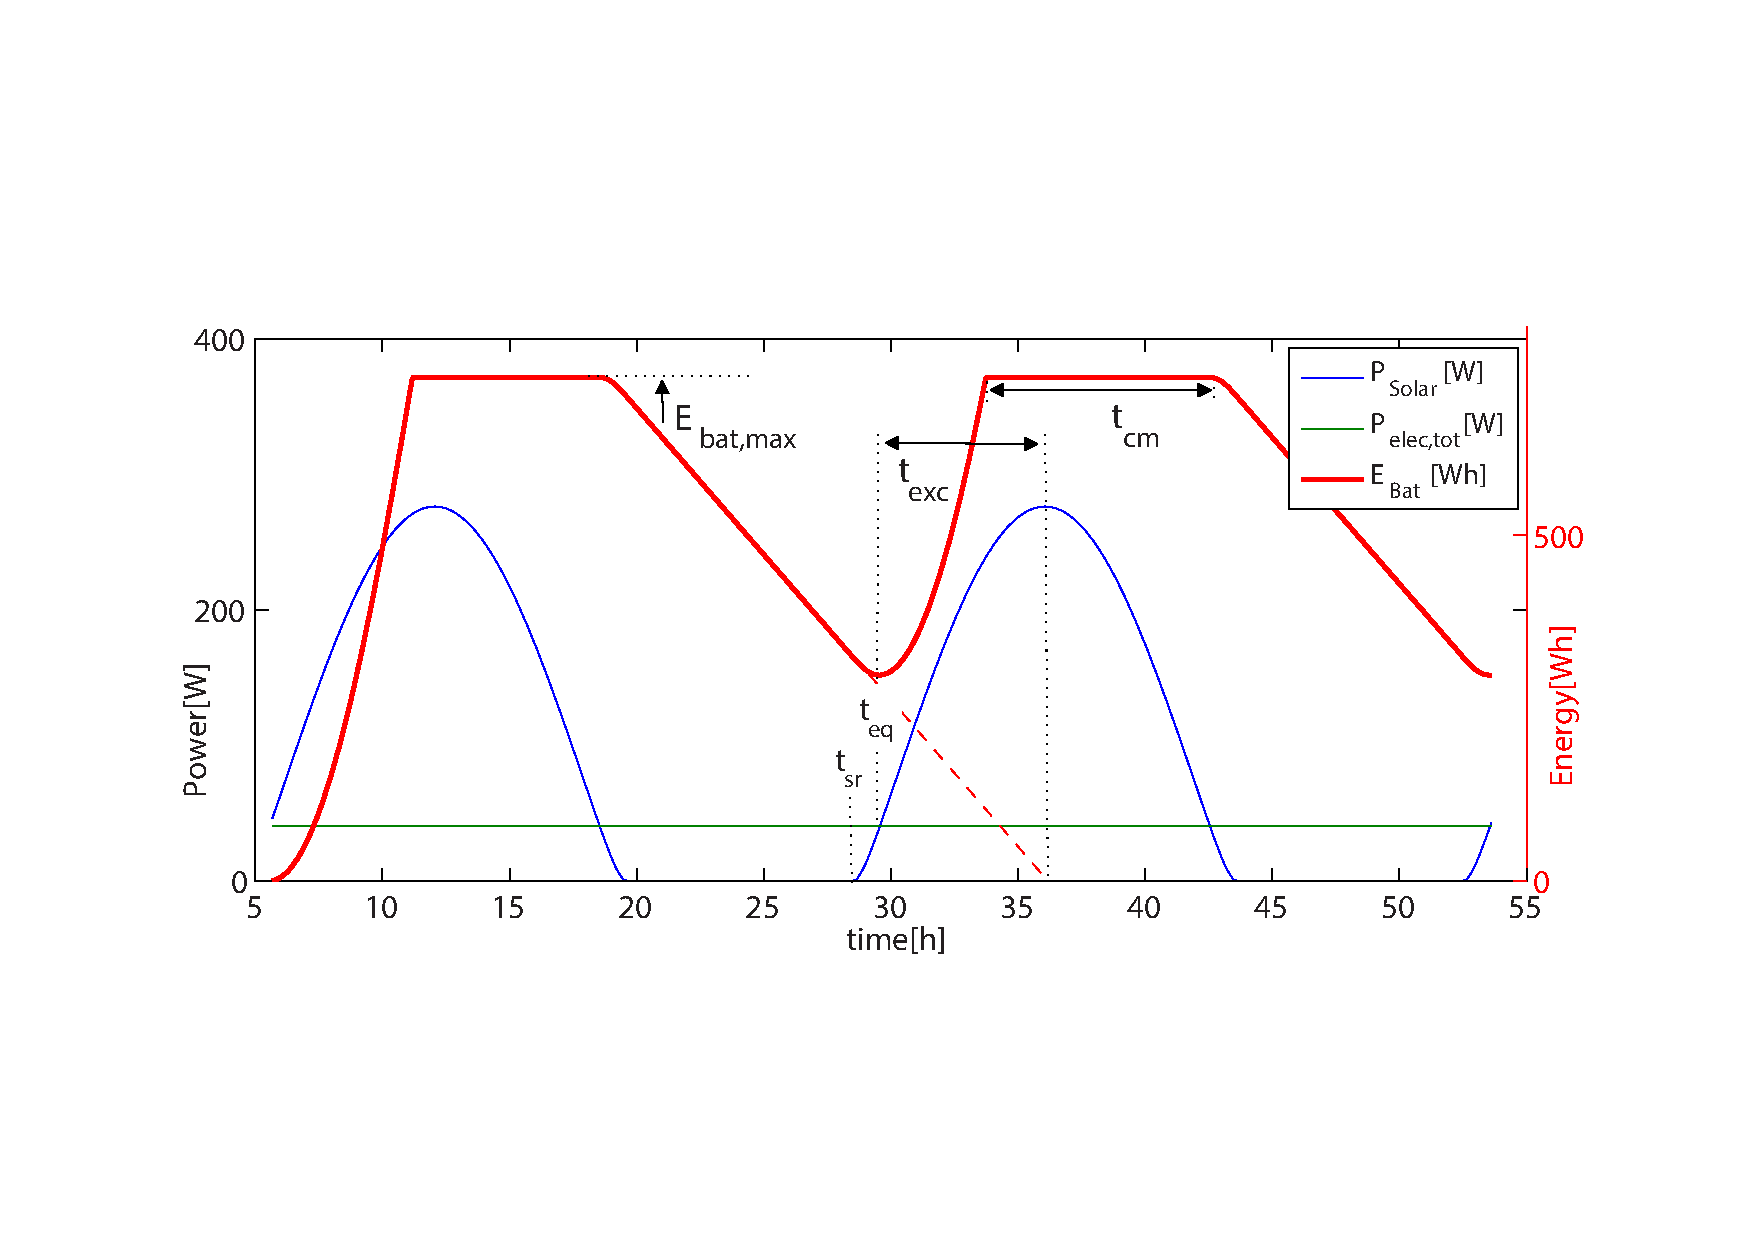
\includegraphics[width=\linewidth]{images/2_EnergySimulation.pdf}
    \caption{Energetic simulation of the AtlantikSolar UAV configuration ($b=5.6m$, $\lambda=18.5$, $m_{bat}=3.5kg$), showing input and output power, battery capacity, and performance metrics excess time $t_{exc}$ and charge margin $t_{cm}$ during a 2-day flight.}
    \label{fig:EnergySimulation}
\end{figure}
Second, and more importantly, the optimization criteria are extended to achieve a more robust multi-day flight. In general, a necessary and sufficient condition for perpetual flight is that the excess time $t_{exc}>0$, where
\begin{equation} \label{eqn:t_exc}
t_{exc}=\frac{E_{bat}(t=t_{eq})}{P_{out}^{\,nom}} \Big| P_{solar}(t>t_{sr})=0
\end{equation}
with \textit{power-equality time} $t_{eq}=t(P_{solar}^{\,nom}=P_{out}^{\,nom})$ in the morning. This means that at $t=t_{eq}$ there has to exist remaining battery capacity to continue flight e.g. in case of cloud coverage. Therefore, the authors in \cite{Noth_PhD,Leutenegger_JIRS} focus on maximizing $t_{exc}$. However, a large $t_{exc}$ does not provide direct robustness against disturbances in $P_{solar}$ e.g. due to cloud coverage during the charging process. In contrast, when optimizing purely for $t_{exc}$, the methodology in Sec. \ref{sec:ConceptualDesignMethodology} will select the largest battery size (due to the scaling of $P_{level}$ with $m_{bat}$) which can be fully charged under optimal conditions, but every reduction in $P_{solar}$ will directly decrease $t_{exc}$ due to only partially charged batteries. Thus, we introduce the charge margin $t_{cm}$ as the time margin between achieving the full charge $E_{bat}=E_{bat}^{\,max}$ and restart of the discharge in the evening. In case of decreased solar power income, $t_{cm}>0$ provides additional margin before a decrease in excess time occurs.

The overall approach for increasing robustness with respect to local power disturbances is thus to determine the lowest acceptable $t_{exc}$ satisfying the UAV application requirements, and then to optimize the configuration for $t_{cm}$. The exact procedure applied is:
\vspace{-3ex}
\begin{algorithm}[htp]
  \SetAlgoLined\DontPrintSemicolon
  \SetKwFunction{proc}{}
  \SetKwProg{myproc}{}{}{}
  \myproc{} %\proc{}
  {
  \nl Choose nominal operating latitude $\varphi$, and Day of Operation $DoY^{nom}$ and the outermost days where perpetual UAV endurance is required $DoY^{\min,\max}$ \;
  \nl For the range of $DoY=[DoY^{\min},DoY^{\max}]$ obtain $t_{night}^{\min},~t_{night}^{\max}$ from~\cite{Duffie_SolarEngineering} \;
  \nl The required excess time $t_{exc,req}$ is now the sum of  \; 
  \pushline
  \nonl \scriptsize$\bullet$\normalsize~  $t_{exc,DoY} = t_{night}^{\,max}-t_{night}^{\,min}$ \;
  \nonl \scriptsize$\bullet$\normalsize~  $t_{exc,clouds}$, to allow a margin for clouds in the morning or evening \;
  \nonl \scriptsize$\bullet$\normalsize~  $t_{exc,P_{level}}$, to allow a margin for increased power consumption e.g. caused by downdrafts or uncertainties in estimating $P_{level}$ \;
  \popline \nl 
  \nl Perform the design analysis given the methodology in Sec.~\ref{sec:ConceptualDesignMethodology} for $DoY(t_{night}=t_{night}^{\,min})$. Pre-select the subset $\pazocal{S}$ of configurations satisfying $t_{exc}>t_{exc,req}$  \;
  \nl Within $\pazocal{S}$, allow for a set of intermediate configurations $\pazocal{S}_i$ to take into account UAV-specific constraints on $b$, $\lambda$, or $m_{bat}$. Then choose the final configuration $\pazocal{S}_f$  from $\pazocal{S}_i$ to obtain the largest charge margin $t_{cm}$ % \; 

 }
  %\caption{Inor}
\end{algorithm}

This conceptual design methodology is applied below. An alternative conceptual design approach utilizing a weighted version of $t_{exc}$ and $t_{cm}$ is proposed in \cite{Morton_ICRA2013}. 

%%%%%%%%%%%%%%%%%%%%%%%%%%%%%%%%%%%%%%%%%%%%%%%%%%%%%%%%%%%%%%%%%%%%%%%%%%%%%%%
\subsection{Application of Conceptual Design Methodology} \label{sec:ConceptDesignApplication}
%%%%%%%%%%%%%%%%%%%%%%%%%%%%%%%%%%%%%%%%%%%%%%%%%%%%%%%%%%%%%%%%%%%%%%%%%%%%%%%

AtlantikSolar operates at a nominal latitude of $\varphi=45\degree N$ and shall provide perpetual endurance within a +/-2 month window around $DoY_{nom}$=June 21\textsuperscript{st} (April 21\textsuperscript{st}-August 21\textsuperscript{st}). From \cite{Duffie_SolarEngineering}, we find $t_{night}^{\,min}=8.7h$ (June 21\textsuperscript{st}), $t_{night}^{\,max}=10.5h$(April 21\textsuperscript{st}), and thus $t_{exc,DoY}=1.80h$. We choose $t_{exc,clouds}=3.0h$ to account for three hours of full cloud coverage either on the evening or the morning and choose $t_{exc,P_{level}}=0.2\cdot t_{night,max}=2.1h$ to cover increased power consumption due to modelling errors, downdrafts or headwinds. Using $t_{exc,req}=t_{exc,DoY}+t_{exc,clouds}+t_{exc,P_{level}}$, we retrieve $t_{exc,req}=6.9h$ as the minimum required excess time for robust perpetual-flight at the given dates and locations. 

The design methodology tool of Sec. \ref{sec:ConceptualDesignMethodology} is now applied assuming the fixed parameters in Tab. \ref{tab:ConceptDesignParameters}. Figure \ref{fig:ExcessTimeChargeMargin} shows the resulting plot for $t_{exc}$ versus the optimization variables $b$ and $m_{bat}$. The subset $\pazocal{S}$ of configurations satisfying $t_{exc}>t_{exc,req}$ is the region within the blue contour-line. The optimum clearly occurs at large wingspans. However, considering that we aim for a small-scale and hand-launchable configuration that allows easy transport (in this case via disassembly of the main wing into three pieces of less than $2m$ wingspan) we choose $b=5.6m$.  The aspect ratio $\lambda=18.5$ is found to provide an optimum in $t_{exc}$ and also allows to seamlessly integrate the 125mm-wide solar cells (see Sec. \ref{secsec:Airframe and hardware}) inside the wing chord. The last design choice is $m_{bat}$, for which we seek to optimize $t_{cm}$ within the previously selected set $\pazocal{S}_i=(\pazocal{S}|b=5.6m, \lambda=18.5)$. As visible in Fig. \ref{fig:ExcessTimeChargeMargin}, $m_{bat}=3.0...7.5kg$ lie within $\pazocal{S}_i$. We choose $m_{bat}=3.5kg$ to optimize $t_{cm}$ and due to practical battery sizing constraints described in Sec. \ref{secsec:Airframe and hardware}. The selected final configuration $\pazocal{S}_f=(\pazocal{S}|m_{bat}=3.5kg, b=5.6m, \lambda=18.5)$ yields an estimated $m_{tot}=7.22kg$, $t_{exc}=7.89h$ and $t_{cm}=8.38h$ for the nominal operating date and latitude.
\begin{figure}[tb]
    \centering
    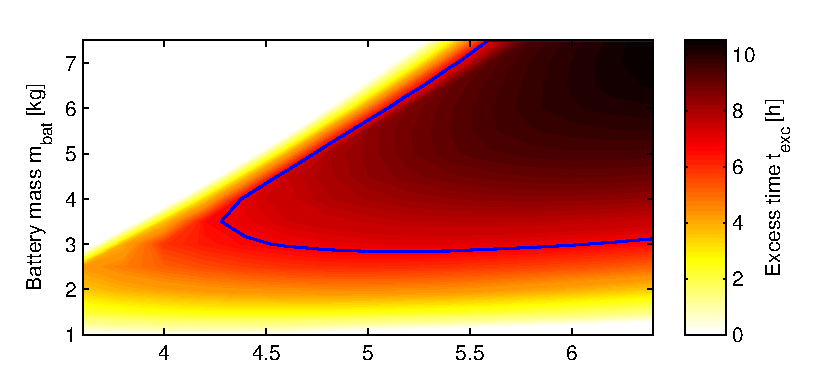
\includegraphics[width=\linewidth]{images/3_excesstime}
    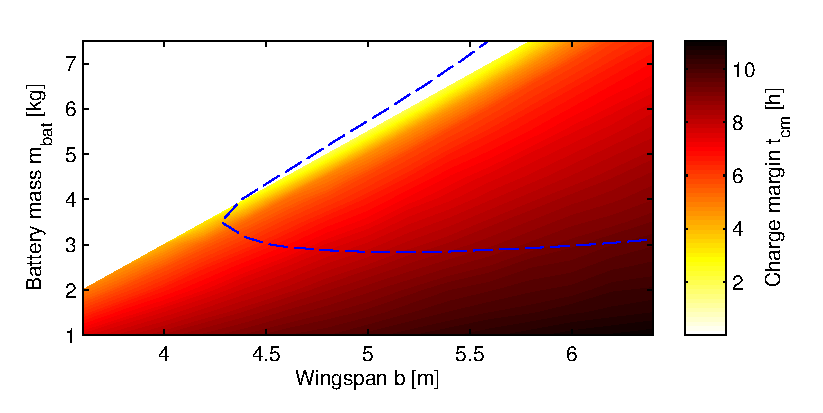
\includegraphics[width=\linewidth]{images/4_chargemargin}
    \caption{Excess time $t_{exc}$ (top) and charge margin $t_{cm}$ (bottom) vs. $b$ and $m_{bat}$, all at $\lambda=18.5$. The configuration subset $\pazocal{S}$ satisfying $t_{exc}>t_{exc,req}$ under our design requirements lies inside the blue contour line.}
    \label{fig:ExcessTimeChargeMargin}
\end{figure}
\begin{table}[h] 
\caption{Fixed parameters for the conceptual design} \label{tab:ConceptDesignParameters}
\begin{center}
\begin{tabular}{l l l}
\toprule
 Parameter & Value & Description\\ 
\midrule
 $\eta_{sm}$ & 0.20&Solar module efficiency\\
 $\eta_{MPPT}$ & 0.97&MPPT efficiency\\
 $\eta_{prop}$ & 0.58 &Propulsion system effiency\\
 $e_{bat}$ & 874800\unitfrac{J}{kg}&Battery specific energy\\
 $f_{sm}$ & 0.94&Solar module fill factor\\
 $k_{sm}$ & 0.59$\unitfrac{kg}{m²}$ & Solar module areal density\\
 $m_{av}$ & 0.6kg&Avionics mass (including all cabling)\\
 $m_{pld}$ & 0.1kg&Payload mass\\
 $P_{av}$ & 4.5\unit{W}&Avionics power consumption\\
 $P_{pld}$ & 0.0\unit{W}&Payload power consumption\\
\bottomrule
\end{tabular}
\end{center}
\end{table}

%%%%%%%%%%%%%%%%%%%%%%%%%%%%%%%%%%%%%%%%%%%%%%%%%%%%%%%%%%%%%%%%%%%%%%%%%%%%%%%
\subsection{Robustness Analysis}
%%%%%%%%%%%%%%%%%%%%%%%%%%%%%%%%%%%%%%%%%%%%%%%%%%%%%%%%%%%%%%%%%%%%%%%%%%%%%%%

To verify the multi-day flight robustness of the developed UAV configuration, we analyze its performance considering a set of local disturbances in UAV power input and output, namely
\begin{itemize}
\item The disturbed solar power income $P_{solar}^{\,dist}$, as caused by clouds or fog. Lacking knowledge of the exact spatial and temporal disturbance distribution, we assume
\begin{equation}
P_{solar}^{\,dist}(t) = P_{solar}^{\,nom}(t) \cdot k_{CCF}.
\end{equation}
Here, $k_{CCF} \in (0,1]$  represents the current cloud cover factor \cite{Kimura_SolarRadAndClouds}, i.e. the clearness of the atmosphere.
\item The disturbed electrical power output $P_{out}^{\,dist}$. Wind downdrafts, head wind, or gusts may require increased propulsion or actuation power. Again, we assume 
\begin{equation}
P_{out}^{\,dist}(t) = P_{out}^{\,nom}(t) \cdot k_{OPF},~k_{OPF} \in (0,1)
\end{equation}
with $k_{OPF}$ representing the Output Power Factor.
\end{itemize}
\begin{figure}
    \centering
    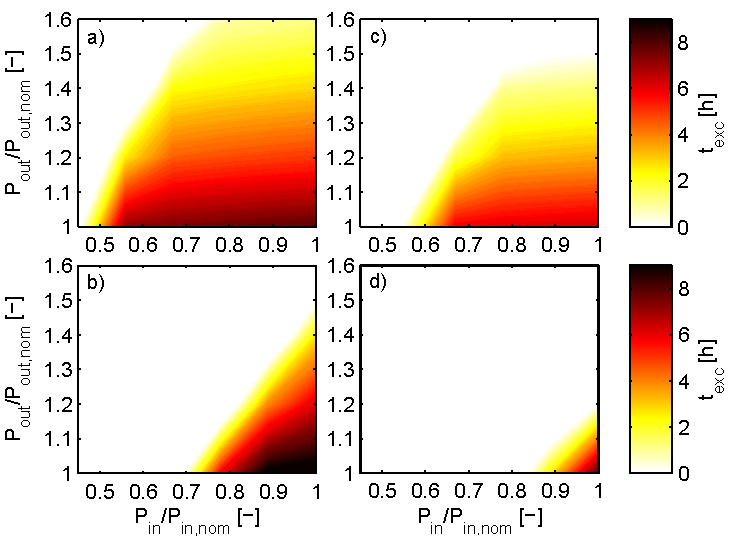
\includegraphics[width=\linewidth]{images/5_texcRobustness/5_texcRobustness.pdf}
    %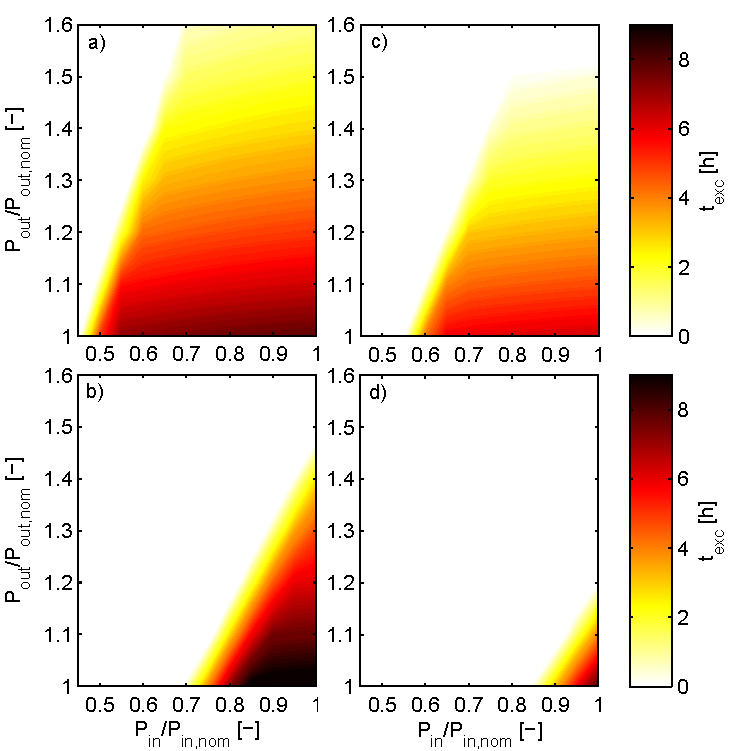
\includegraphics[width=\linewidth]{images/old/5_texcRobustness.pdf}
    \caption{Excess time under disturbed power input and output for the $b=5.6m$, $\lambda=18.5$ configuration: a) $m_{bat}$=3.5kg on June 21\textsuperscript{st} b) $m_{bat}=6.0kg$ on June 21\textsuperscript{st} c) $m_{bat}$=3.5kg on April 21\textsuperscript{st} d) $m_{bat}=6.0kg$ on April 21\textsuperscript{st} }
    \label{fig:ExcessTimeRobustness}
\end{figure}
Fig. \ref{fig:ExcessTimeRobustness} shows the remaining excess time with respect to these disturbances. The UAV configuration developed in Section \ref{sec:ConceptDesignApplication} ($m_{bat}=3.5kg$) still provides perpetual endurance with less than 50\% of the solar power income or if more than 60\% surplus power are required on June 21\textsuperscript{st} (Fig. \ref{fig:ExcessTimeRobustness}a). In contrast, a configuation purely optimized towards excess time ($m_{bat}=6.0kg$, Fig. \ref{fig:ExcessTimeRobustness}b) will yield a higher maximum $t_{exc}$ of 9.5h, but the robustness with respect to clouds or higher required level power is greatly decreased. On April  21\textsuperscript{st}, the UAV configuration of Section \ref{sec:ConceptDesignApplication} still provides solid robustness (Fig. \ref{fig:ExcessTimeRobustness}c), which verifies the $DoY^{\,nom}\pm$ 2 months perpetual endurance requirement. In contrast, the $m_{bat}=6.0kg$ configuration (Fig. \ref{fig:ExcessTimeRobustness}d) can not provide reliable perpetual endurance anymore. Overall, the configuration developed using the extended optimization criteria from Sec. \ref{sec:ExtensionOptCriteria} thus shows significantly improved multi-day flight robustness in comparison with configurations that are purely optimized for maximum excess time.